
\appendix{Additional figures\label{appendix:sample}}
Area Under the Curve (AUC) measures the accuracy or performance of the model with different thresholds. To calculate ROC and area under curve (AUC) we need a True positive rate (TPR) and a False negative rate (FPR). 

\(TPR = \frac{TruePositive}{TruePositive + FalseNegative}\)
\(FPR = \frac{FalsePositive}{FalsePositive + TrueNegative}\)


\begin{table}[h]
\begin{tabular}{ll|ll|}
\cline{3-4}
 &  & \multicolumn{2}{l|}{Actual}              \\ \cline{3-4} 
 &  & \multicolumn{1}{l|}{Positive} & Negative \\ \hline
\multicolumn{1}{|l|}{\multirow{2}{*}{Predicted}} & Positive & \multicolumn{1}{l|}{True Positive}  & False Positive \\ \cline{2-4} 
\multicolumn{1}{|l|}{}                           & Negative & \multicolumn{1}{l|}{False Negative} & True Negative  \\ \hline
\end{tabular}
\end{table}

\begin{figure}[h]
    \centering
    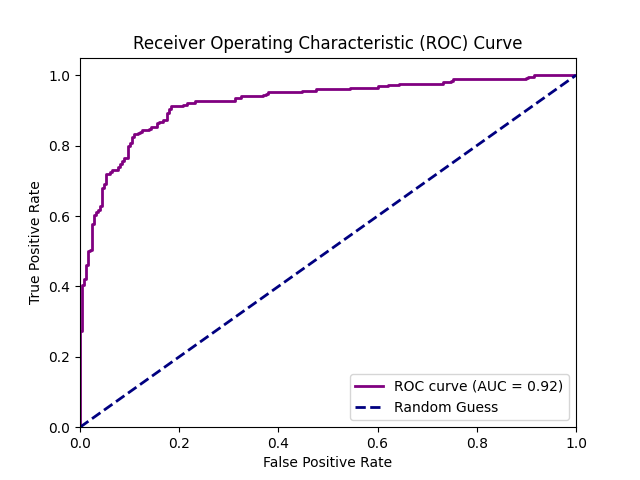
\includegraphics[width=1\linewidth]{template//figures/roc_curve_example1.png}
    \caption{AUC and ROC example}
    \label{fig:enter-label}
\end{figure}




\begin{figure}[h]
    \centering
    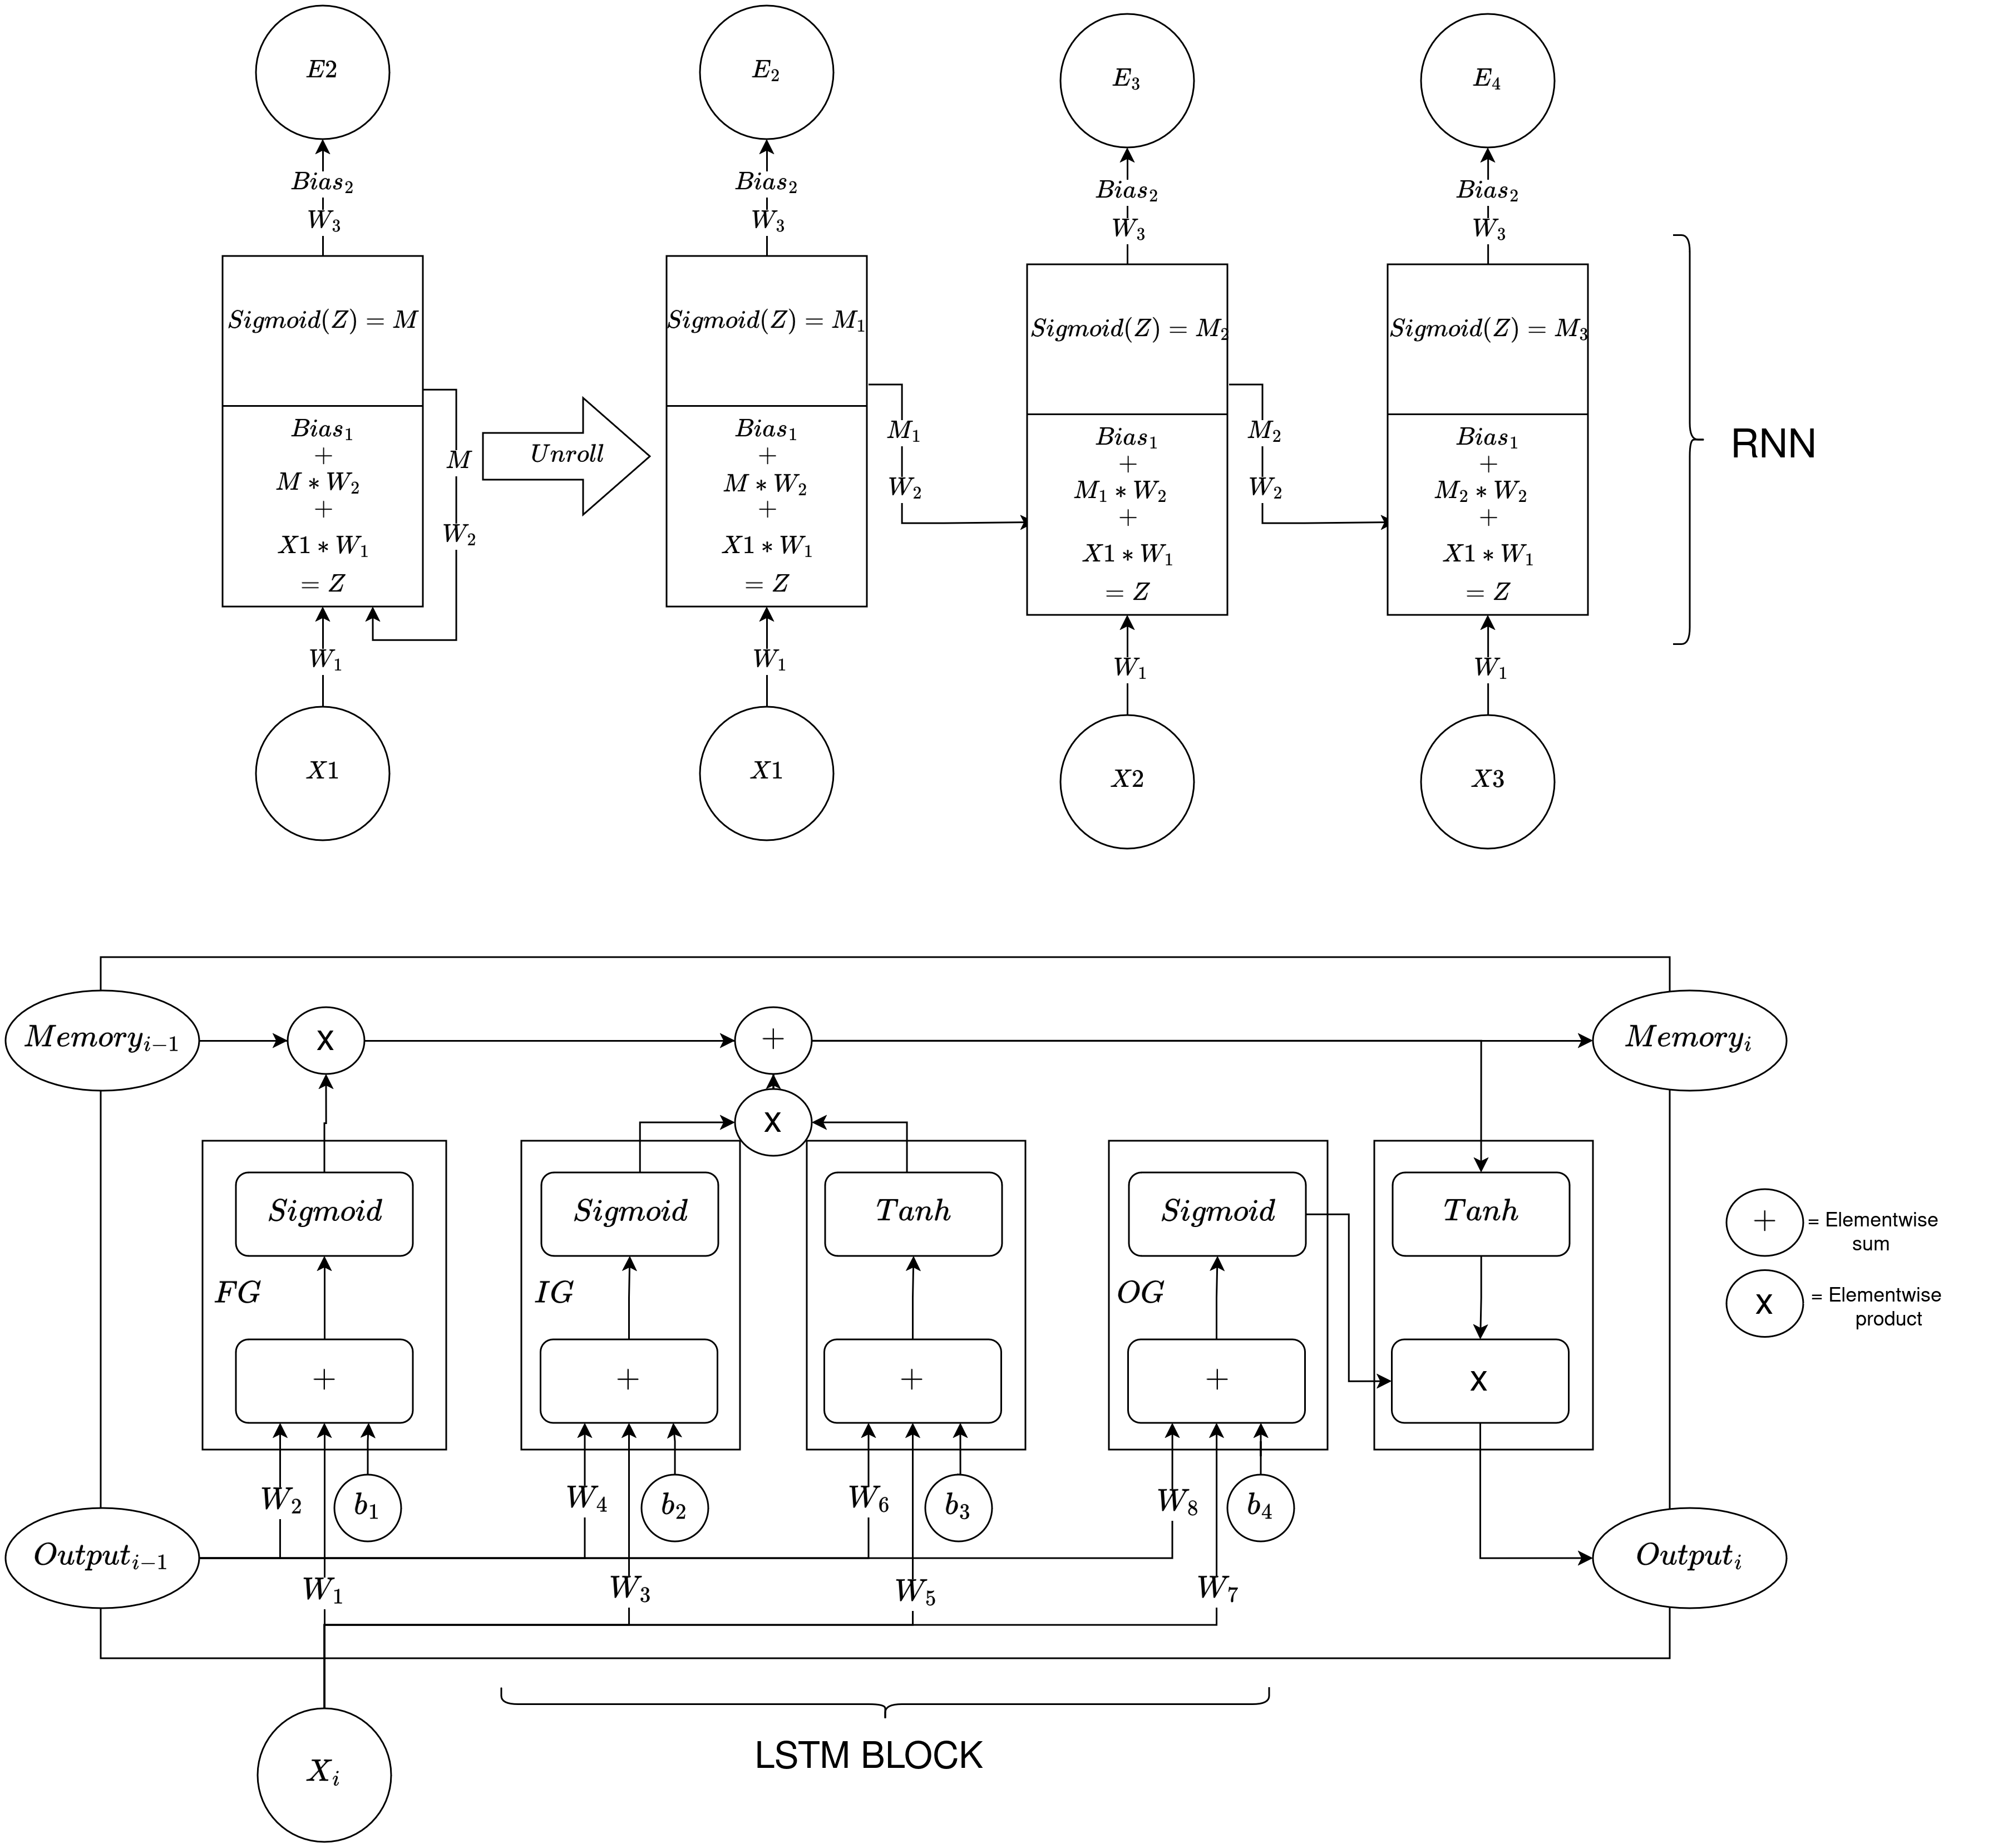
\includegraphics[width=1\linewidth]{template//figures/RNNEXPL_R.png}
    \caption{Sturcture of RNN and LSTM illustrated [inspired: (\cite{googleblog})]}
    \label{RNNEXPL}
\end{figure}

